\chapter{Implementation}



\section{Software Components}
The following examples are made in order to show the modularity of the system:
\begin{itemize}
	\item Filter
	\item Grab with metadata from file
	\item Consumer taking data from snapshot and providing dynamic metadata

\end{itemize}

\section{Metadata profile} \label{sec:design:metadataprofile} 
A profile must be defined, in order to define a new set of parameters for the RTP packet, in order to use the RTP to carry metadata and events. These parameters are listed below:

\begin{itemize}
	\item \textbf{Packet type}: In the metadata profile, the \textit{Packet type}-field will be used to tell which format the metadata is in. Only two  dataformats are defined, however the RTP profile allows up to $2^7=128$  packet types.
		\begin{itemize}
			\item 0: SDP file. the payload of the RTP packet is in the SDP format.
			\item 1: Perl hashmaps. The payload of the RTP packet is a dump of a perl hashmap. This allows a sender to dump a hashmap of key-value pairs and reconstruct the hashmap on the recipient.
			\item 2: JSON. The payload of the RTP packets are JSON encoded. Each RTP packet contain valid JSON encoded data.
		\end{itemize}
	\item \textbf{Marker bit}: The \textit{Marker}-bit is used to denote whether the RTP packet announces a new frame or provides metadata.
		\begin{itemize}
			\item 0, the RTP packet announces a stream. How the payload is encoded is specified by the \textit{Packet Type}-field.
			\item 1, the RTP packet contains an event. How the content of the packet is encoded is specified by the \textit{Packet Type}-field.
		\end{itemize}
	\item \textbf{32 bit timestamp}
\end{itemize}


\section{RTP Libraries}
\subsection{oRTP} 
The oRTP library is used in \textit{linphone Open-source VoIP}, which is an open-source VoIP solution created and maintained by Belledonne Communications. The oRTP library is released under the GNU GPLv2 and proprietary license meaning the library can be used for open-source projects and in proprietary solutions.
The oRTP library implements RFC3550 with an API that offers a high as well as low level API. The library supports parsing and composing RTP and RTCP packets. It supports multiple RTP sessions with IPv4 and IPv6. Furthermore, it offers support for different profiles, meaning a custom profile can be implemented.  oRTP has a sparse documentation with only an autogenerated doxygen, where most of the functionality is described. The sourcecode comes with simple examples, that explains some of the library functionality. The library is written in C, meaning language bindings can be utilized to interface the library to scripting languages. The oRTP library can be found in ubuntu + debian's packet repository. At the time of writing, the latest commit on their official github has been made 24 days ago which indicates the project is active.

\subsection{jrtplib}
The jrtplib library is developed at the the Expertise Centre for Digital Media (EDM), a research institute of the Hasselt University. At the time of writing the library has been used in 61 projects listed on \href{http://research.edm.uhasselt.be/jori/cgi-bin/listprojects.py?name=jrtplib}{Project list}. The library is free to use, but must include disclaimer in the source. The library implements RFC3550 and provides primarily a highlevel API, that hides most of the implement details. The library is written in C++, which allows for language bindings. The library is  well documented by giving a thoroughly \textit{Getting Started} and includes 7 examples showing how to utilize the functionality of the library. Unfortunately the author has not done any commits for the past year.

\todo{MIT license}
\todo{Add to design requirements, that software exist from repo + maintained}
\todo{Explain \textit{library properties}}

\begin{table}[h!]
\centering
\begin{tabular}{@{}|l|l|l@{}|}
\hline
\multicolumn{1}{|l|}{\textbf{Library property}} & \multicolumn{1}{|l|}{\textbf{oRTP}}         & \multicolumn{1}{|l|}{\textbf{jrtplib}}       \\ \midrule
\multicolumn{1}{|l|}{In repository}    & \multicolumn{1}{c|}{\checkmark} & \multicolumn{1}{l|}{} \\ \midrule
\multicolumn{1}{|l|}{RTCP impl.} & \multicolumn{1}{c|}{\checkmark} & \multicolumn{1}{c|}{\checkmark} \\ \midrule
\multicolumn{1}{|l|}{Low level API} & \multicolumn{1}{c|}{\checkmark} & \multicolumn{1}{c|}{\checkmark} \\ \midrule
\multicolumn{1}{|l|}{RTP Profile} & \multicolumn{1}{c|}{\checkmark} & \multicolumn{1}{c|}{\checkmark} \\ \midrule
\multicolumn{1}{|l|}{API documented}          & \multicolumn{1}{c|}{\checkmark} & \multicolumn{1}{c|}{\checkmark} \\ \midrule
\multicolumn{1}{|l|}{Library Usage}          & \multicolumn{1}{c|}{\checkmark} & \multicolumn{1}{c|}{\checkmark} \\ \midrule
\multicolumn{1}{|l|}{Actively Maintained}           & \multicolumn{1}{c|}{\checkmark} & \multicolumn{1}{l|}{} \\ \midrule
\multicolumn{1}{|l|}{IPv6 multicast support}           & \multicolumn{1}{c|}{\checkmark} & \multicolumn{1}{c|}{\checkmark} \\ \midrule
\multicolumn{1}{|l|}{Existing perl-binding}           & \multicolumn{1}{c|}{\checkmark} & \multicolumn{1}{c|}{\checkmark} \\ \midrule
\multicolumn{1}{|l|}{Multiple RTP sessions support}           & \multicolumn{1}{c|}{\checkmark} & \multicolumn{1}{c|}{\checkmark} \\ \midrule
\multicolumn{1}{|l|}{Send \& Receive}           & \multicolumn{1}{c|}{\checkmark} & \multicolumn{1}{c|}{\checkmark} \\ \midrule
\multicolumn{1}{|l|}{Includes examples}           & \multicolumn{1}{c|}{\checkmark} & \multicolumn{1}{c|}{\checkmark}  \\ \bottomrule
\end{tabular}
\caption{Comparesion of oRTP and jrtplib}
\label{my-label}
\end{table}


Comparison of rtpdump(rtptools) and tcpdump+tcpreplay.

% Please add the following required packages to your document preamble:
% \usepackage{graphicx}
\begin{table}[H]
\centering
\resizebox{\textwidth}{!}{%
\begin{tabular}{|l|c|c|}
\hline
\textbf{}       & \textbf{tcpdump/tcpreplay} & \textbf{rtpdump/rtpplay} \\ \hline
Record duration &                            &                          \\ \hline
IPv6 support    & \checkmark  & X                        \\ \hline
Multiple replay &                            &                          \\ \hline
Replay of RTCP  &          \checkmark                 &         X                 \\ \hline
\end{tabular}%
}
\caption{My caption}
\label{my-label}
\end{table}


\section{Test}
From wireshark after resample:
4096 = payload
8 bytes = data gram
12 bytes rtp header

4116 bytes i total

Compare output of stream with snapshot-file
Write 1XXXE and verify with wireshark dissector
    - in table with output
Two subscribers to one stream - compare data. \# samples, md5 of files.
Record and replay, plot to verify data
Compare RTCP abs. timestamp with expected timestamp form RTP samples.

\section{Timing in RTCP packets}
\begin{align}
	mon_1 &= Monotonic time \\
	realtime &= now \\
	mon_2 &= Monotonic time \\
	offset &= realtime-(mon_1+mon_2)/2 
\end{align}


\section{Ipv6}
   IPv6 sessions are announced on the address FF0X:0:0:0:0:0:2:7FFE
      where X is the 4-bit scope value.  For example, an announcement
      for a link-local session assigned the address
      FF02:0:0:0:0:0:1234:5678, should be advertised on SAP address
      FF02:0:0:0:0:0:2:7FFE.
      

Generation of random IPv6:
Last part of IPv6:
::XXXX = 16 bits
$2^16 = 65536$
 \todo{Compare gstreamer with custom impl.}


\section{Gstreamer}
Gstreaner is a open source tool available, that implements some of the protocols described in section \ref{sec:design:protocols}.
\todo{Describe gstreamer + pros and cons}
Cons:
 - 64bit timestamp injected
 - Does not handle multicast address assignment
Gstreamer is a pipeline based streaming framework that aims to make it easy to work with streams. Gstreamer is plugin based which allows for adding functionality as needed in applications. The idea of plugins is to create plugins are have a well defined responsibility such as reading a file, encoding, playing etc. The plugins are usually connected in gstreamer pipelines, however then can be used in independent applications. Gstreamer plugins are connected using pads, where each plugin can have a source and sink pad. A source pad can then be connected to the next plugin's sink pad. An example of plugins in a pipelines is showed below:
\begin{figure}
	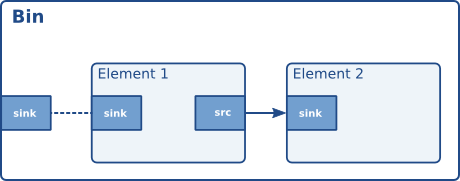
\includegraphics[width=1\textwidth]{figures/bin-element-ghost.png}
\end{figure}

\todo{Describe example figure + rtpbin + rtppay/depay}

\todo{Describe dummy producer.pl}
\section{Only permit one publisher pr. stream}

The test has been conducted by first starting one instance of \program{Publisher} and when it starts to publish data, then a second instance of the \program{Publisher}. Both \program{Publishers} have been given the same highbandwidth IPv6 multicast address, namely FF15::1234.

Listing \ref{lst:implementation:uniquepub1} shows the output from the first \program{Publisher}.

\begin{lstlisting}
Random ip: ff15::1234
Verbose: 5
Executable: producer.pl
"producer.pl" is readable
"producer.pl" is exeutable
Data pipe: /tmp/pipe_publisher_data metadata pipe:/tmp/pipe_publisher_metadata
Waitfor: duration 5.000000 and interval 1.000000
Callback invoked...
Waitfor: wake from sleep at elapsed 1.000000
Callback invoked...
Waitfor: wake from sleep at elapsed 2.000000
Callback invoked...
Waitfor: wake from sleep at elapsed 3.000000
Callback invoked...
Waitfor: wake from sleep at elapsed 4.000000
Callback invoked...
Waitfor: wake from sleep at elapsed 5.000000
Waitfor: loop completed, elapsed 5.000000 of 5.000000
No IPv6 multicast conflict
\end{lstlisting} \label{lst:implementation:uniquepub1}

Listing \ref{lst:implementation:uniquepub2} shows the output from the second instance of the \program{Publisher}.

\begin{lstlisting}
Random ip: ff15::1234
Verbose: 4
Executable: producer.pl
"producer.pl" is readable
"producer.pl" is exeutable
Data pipe: /tmp/pipe_publisher_data metadata pipe:/tmp/pipe_publisher_metadata
Waitfor: duration 5.000000 and interval 1.000000
Callback invoked...
ff15::1234 vs. ff15::1234
Waitfor: loop completed, elapsed 1.000000 of 5.000000
Ipv6 multicast group conflict
New random IPv6 multicast ip: ff15::8a12
Waitfor: duration 5.000000 and interval 1.000000
Callback invoked...
ff15::1234 vs. ff15::8a12
Callback invoked...
ff15::1234 vs. ff15::8a12
Callback invoked...
ff15::1234 vs. ff15::8a12
Callback invoked...
ff15::1234 vs. ff15::8a12
Callback invoked...
ff15::1234 vs. ff15::8a12
Waitfor: loop completed, elapsed 5.000000 of 5.000000
No IPv6 multicast conflict
\end{lstlisting}\label{lst:implementation:uniquepub2}


